\chapter{История}							% Заголовок
\addcontentsline{toc}{chapter}{История}	% Добавляем его в оглавление

История создания шагающих механизмов очень богата и уходит в глубокую древность. Одно из первых упоминаний в литературных источниках (Reconstruction designs of lost ancient Chinese machinery" By Hong-Sen Yan ,http://cyberneticzoo.com/walking-machines/480-bc-wooden-horse-carriage-lu-ban/) датируется 480 годом до нашей эры - деревянная лошадь с повозкой, автор --- Лю Бан, Китай. Современную репродукцию лошади с повозкой можно видеть на рис. \ref{img:wooden_horse}.

\begin{figure}[ht]
	\begin{minipage}[ht]{0.49\linewidth}
		\centering{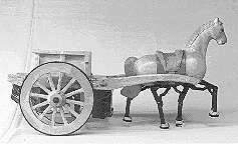
\includegraphics[width=0.8\linewidth]{Introduction/intro1} \\ а)}
	\end{minipage}
	\hfill
	\begin{minipage}[ht]{0.49\linewidth}
		\centering{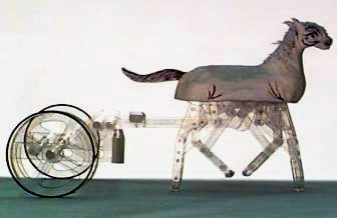
\includegraphics[width=0.8\linewidth]{Introduction/intro2} \\ б)}
	\end{minipage}
	\caption{Деревянная лошадь с повозкой, 480 год до н.э. Лю Бан, Китай}
	\label{img:wooden_horse}  
\end{figure}

Одним из первых ученых нового времени, заинтересовавшихся задачей математического анализа перемещения стопоходящих животных, стал известный русский математик и механик П.Л. Чебышев. В 1878 г. на Всемирной выставке в Париже была продемонстрирована так называемая стопоходящая машина, имитирующая движение четырехногого животного при ходьбе. Кинематическая схема машины состоит из четырех лямбда-механизмов Чебышева. В настоящее время действующая реплика машины хранится в московском Политехническом музее. Модель стопоходящей машины изображена на рис. \ref{img:chebishev}

\begin{figure}[ht]
	\centering
	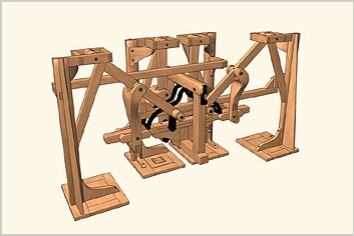
\includegraphics[width = 0.5\linewidth]{Introduction/intro3}
	\caption{Стопоходящая машина П.Л. Чебышева. 1878 г}
	\label{img:chebishev}
\end{figure}

П.Л. Чебышев является одним из основоположников математической теории синтеза механизмов.

В СССР исследования по тематике шагающих роботов начинались в ИМАШ АН СССР в ИПМ АН СССР (позднее ИПМ им.М.В.Келдыша РАН). В ИПМ АН СССР работы велись под руководством Д.Е. Охоцимского. В периода 1972-1975гг были созданы первые макеты многоногих шагающих машин. На рис. \ref{img:imash_ran}

\begin{figure}[ht]
	\centering
	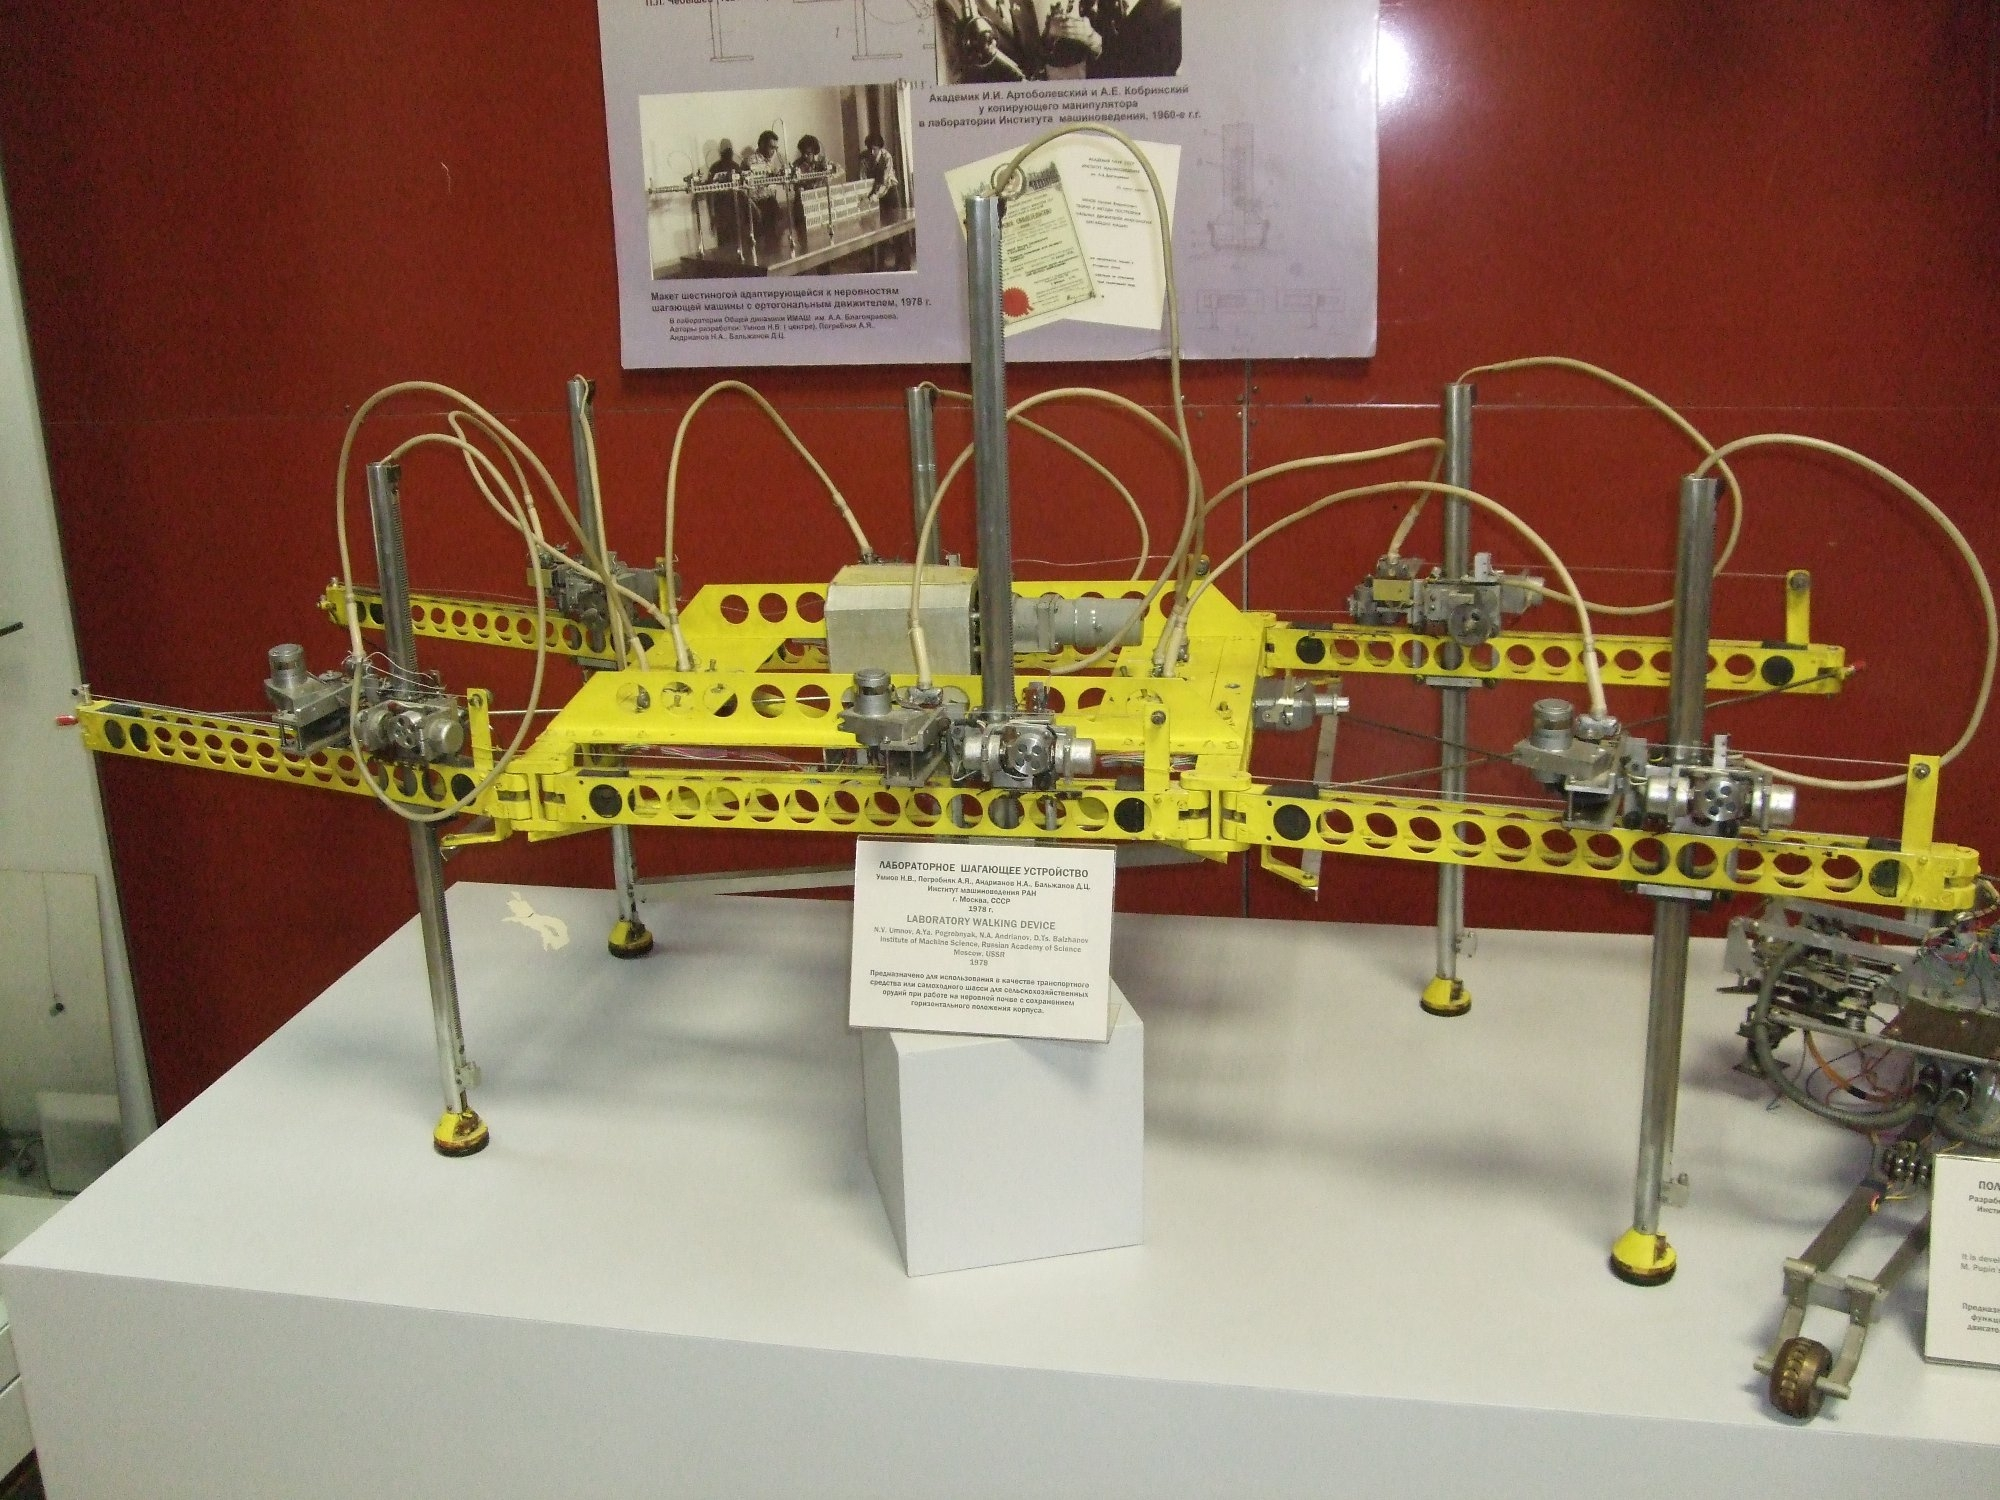
\includegraphics[width = 0.5\linewidth]{Introduction/intro4}
	\caption{Шагающая машина ИМАШ РАН}
	\label{img:imash_ran}
\end{figure}

В шагающем аппарате ИМАШ РАН использована оригинальная кинематика ног --- ортогональная. Каждая из шести ног состоит из пары штоковых механизмов, соединенных между собой под прямым углом. Один из штоков жестко крепится к корпусу, второй шток используется для удержания веса аппарата. Преимущество данной ортогональной кинематики ноги состоит в простом синтезе движения.

На рис. \ref{img:IPM_robots} изображены макеты шестиногих шагающих аппаратов, созданных в Институте Прикладной Математики АН СССР.

\begin{figure}[ht]
	\begin{minipage}[ht]{0.49\linewidth}
		\centering{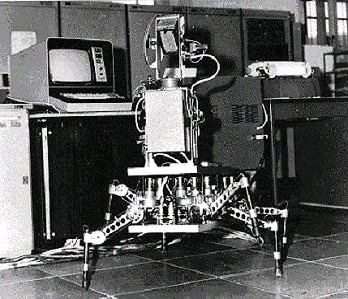
\includegraphics[width=0.5\linewidth]{Introduction/intro5} \\ а)}
	\end{minipage}
	\hfill
	\begin{minipage}[ht]{0.49\linewidth}
		\centering{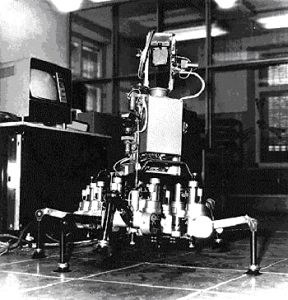
\includegraphics[width=0.5\linewidth]{Introduction/intro6} \\ б)}
	\end{minipage}
	\caption{Шагающие роботы ИПМ АН СССР. Фото 1975г}
	\label{img:IPM_robots}  
\end{figure}

Аппараты оснащены инсектоморфными (насекомоподобными, от англ. insect --- насекомое) ногами. Каждая нога обладает тремя степенями подвижности. На рисунке \ref{img:IPM_robots} аппараты оснащены лазерным измерителем расстояний --- ЛИР. С помощью ЛИР система управления робота получала информацию об окружающем пространстве и принимала решение о параметрах движения. Наличие шести ног позволяет аппарату передвигаться статически устойчивой походкой. Именно наличие множества классов статически устойчивых походок определило интерес к многоногим машинам.

В результате совместных работ ИПМ им М.В. Келдыша АН СССР и ВНИИТРАНСМАШ в 1975г создан макет шестиногой шагающей машины НМША (Натурный Макет Шагающего Аппарата) способной нести на себе человека оператора-водителя. Масса машины составляет 750кг, скорость движения 0,7 км/ч, грузоподъемность 50кг, дорожный просвет 1,5 м. Аппарат НМША изображен на рис. \ref{img:NMSHA}

\begin{figure}[ht]
	\begin{minipage}[ht]{0.49\linewidth}
		\centering{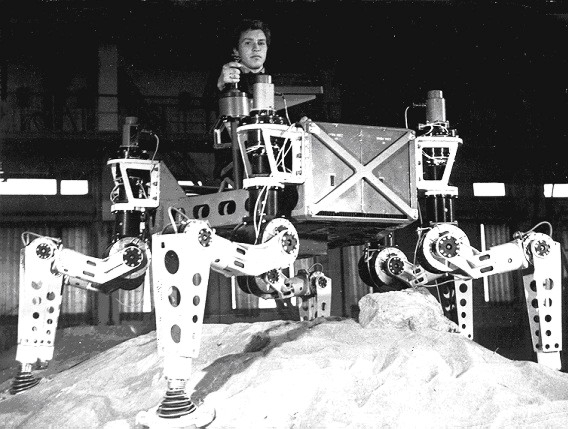
\includegraphics[width=0.8\linewidth]{Introduction/intro7} \\ а)}
	\end{minipage}
	\hfill
	\begin{minipage}[ht]{0.49\linewidth}
		\centering{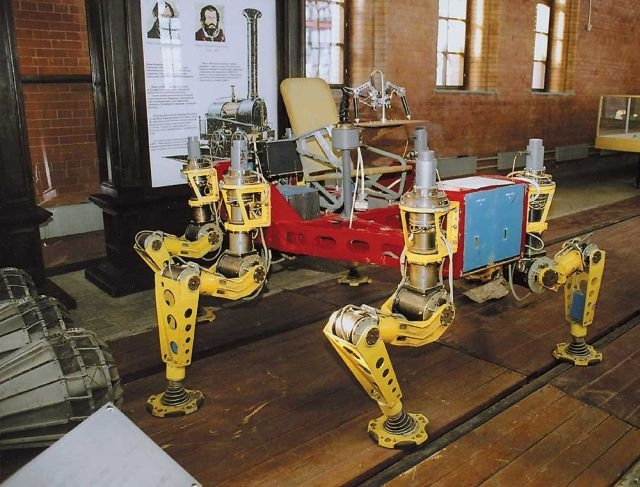
\includegraphics[width=0.8\linewidth]{Introduction/intro8} \\ б)}
	\end{minipage}
	\caption{Аппарат НМША. 1975г}
	\label{img:NMSHA}  
\end{figure}

Обозначенные исследования на базе ИПМ им.М.В.Кледыша продолжаются в настоящее время. На рис. \ref{img:IPM_now} показан макет робота третьего поколения. На роботе установлены современные электродвигатели, бортовая процессорная система управления. На аппарате установлен необходимый набор сенсоров и датчиков.

\begin{figure}[ht]
	\begin{minipage}[ht]{0.49\linewidth}
		\centering{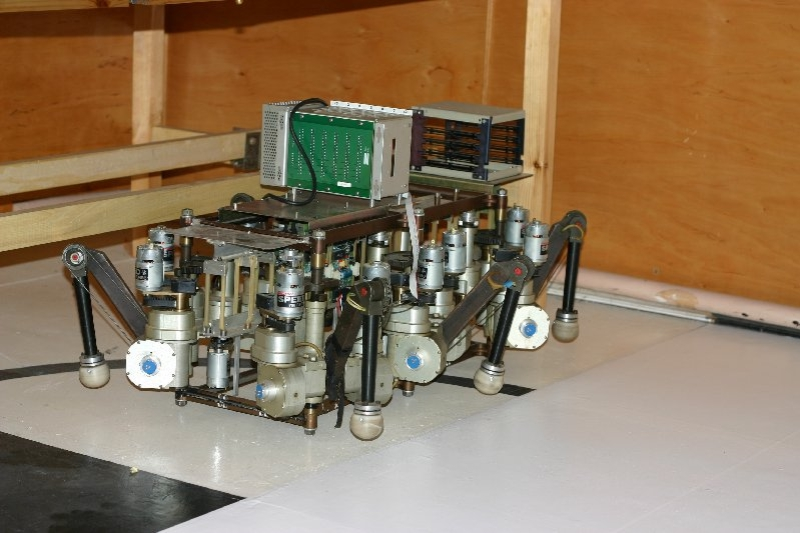
\includegraphics[width=0.8\linewidth]{Introduction/intro9} \\ а)}
	\end{minipage}
	\hfill
	\begin{minipage}[ht]{0.49\linewidth}
		\centering{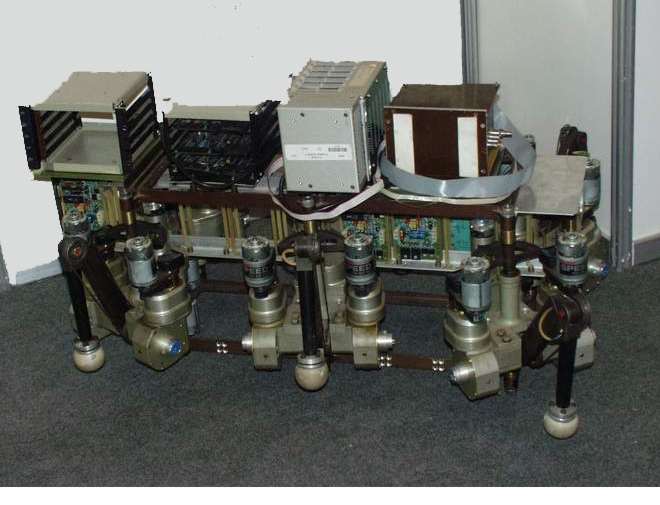
\includegraphics[width=0.8\linewidth]{Introduction/intro10} \\ б)}
	\end{minipage}
	\caption{Шагающий робот ИПМ им.М.В.Келдыша РАН. Фото 2009 г}
	\label{img:IPM_now}  
\end{figure}

Работы по исследованию шагающих аппаратов ведутся в Институте Механики МГУ. На рис. \ref{img:masha} изображен макет шагающего робота МАША --- МАшина ШАгающая.

\begin{figure}[ht]
	\begin{minipage}[ht]{0.49\linewidth}
		\centering{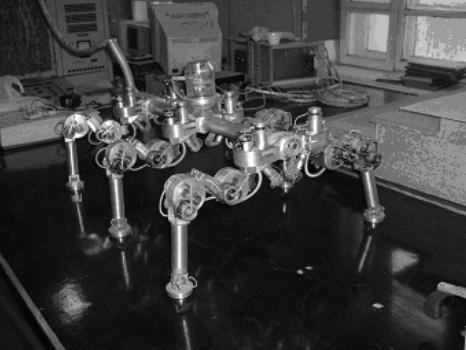
\includegraphics[width=0.8\linewidth]{Introduction/intro11} \\ а)}
	\end{minipage}
	\hfill
	\begin{minipage}[ht]{0.49\linewidth}
		\centering{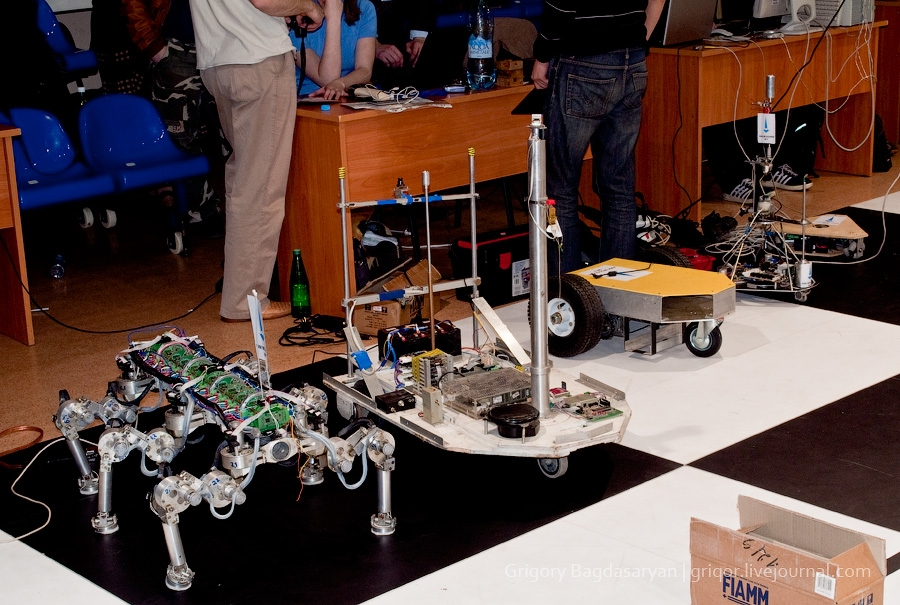
\includegraphics[width=0.8\linewidth]{Introduction/intro12} \\ б)}
	\end{minipage}
	\caption{МАША. Институт Механики МГУ.}
	\label{img:masha}  
\end{figure}

Проекты шагающих машин выполнены практически во всех технологически развитых странах. Приведем примеры иностранных разработок.

Одним из первых шагающих аппаратов в США является так называемая Калифорнийская лошадь --- Phoney Poney. Фотография макета изображена на рис. \ref{img:phoney_poney}

\begin{figure}[ht]
	\centering
	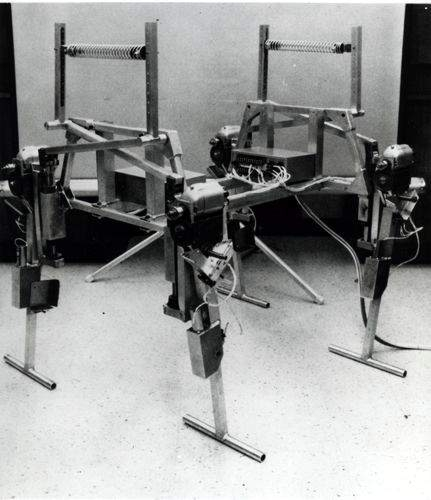
\includegraphics[width = 0.4\linewidth]{Introduction/intro13}
	\caption{Калифорнийская лошадь --- Phoney Pony. Университет Южной Калифорнии, 1968 г }
	\label{img:phoney_poney}
\end{figure}

Аппарат разработан и собран аспирантом Andrew Frank, под руководством профессора Robert McGhee в Университете Южной Калифорнии в 1968 году. Аппарат мог передвигаться рысью, галопом и другими походками четвероногих. Для управления робота использовалась ЭВМ размером с комнату, а управление осуществлялось по отдельному кабелю. Калифорнийская лошадь является первым примером практического применения теории конечных автоматов для управления движением шагающего аппарата.

На рис. \ref{img:walking_truck} изображена машина компании General Electric (США) ---  Walking Truck (Шагающий грузовик). Управление аппарата построено на копирующих манипуляторах. Оператор-водитель при помощи рук и ног передает движение через копирующие механизмы на соответствующие конечности аппарата.

\begin{figure}[ht]
	\centering
	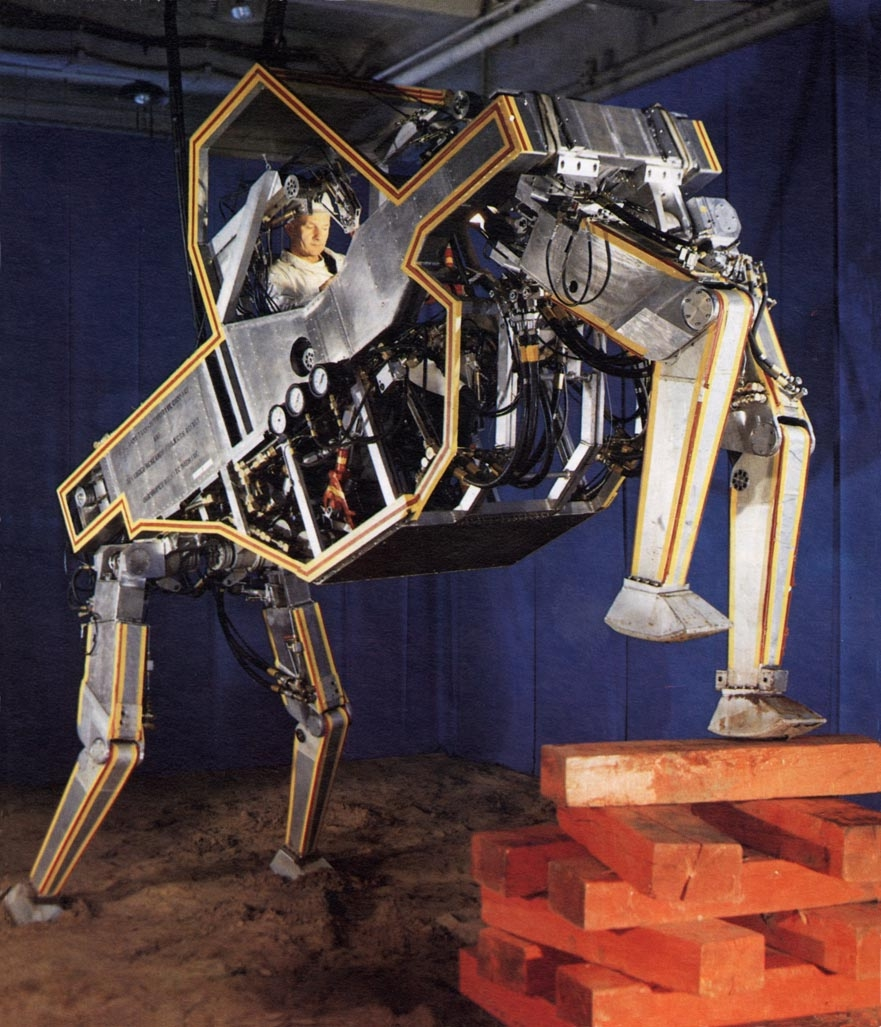
\includegraphics[width = 0.5\linewidth]{Introduction/intro14}
	\caption{General Electrick Walking Truck, США, 1969 г}
	\label{img:walking_truck}
\end{figure}

Шагающий грузовик разрабатывался для нужд Министерства Обороны США. Предполагалось использовать Шагающий грузовик в труднопроходимых местах для перевозки военного оборудования, аммуниции, людей. Система управления аппарата оказалась слишком сложной для человека --- требовала от оператора-водителя огромного напряжения внимания и сил. Стало очевидным, что часть низкоуровневых функций управления, таких как координация движений ног аппарата и поддержание устойчивого положения аппарата, нужно перекладывать с человека на автоматику.

На следующих фотографиях изображены разработки второй половины ХХ века.

\begin{figure}[ht]
	\centering
	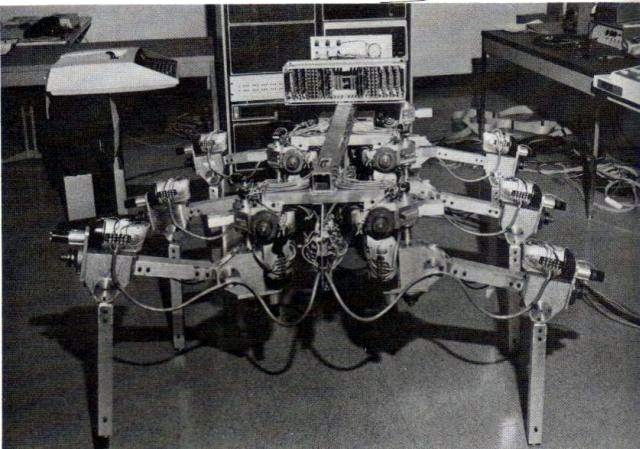
\includegraphics[width = 0.5\linewidth]{Introduction/intro15}
	\caption{Шетсиногий шагающий аппарат. Университет Огайо, профессор Robert McGhee. США}
	\label{img:intro15}
\end{figure}

\begin{figure}[ht]
	\begin{minipage}[ht]{0.49\linewidth}
		\centering{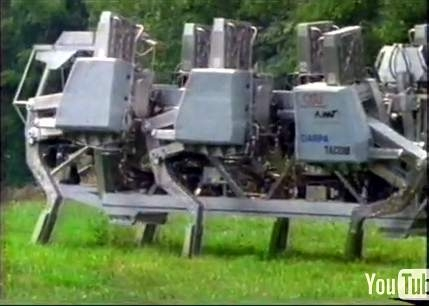
\includegraphics[width=0.8\linewidth]{Introduction/intro16} \\ а)}
	\end{minipage}
	\hfill
	\begin{minipage}[ht]{0.49\linewidth}
		\centering{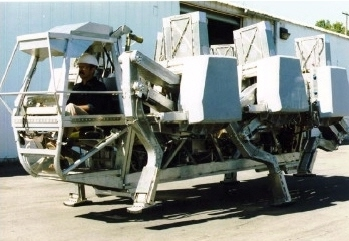
\includegraphics[width=0.8\linewidth]{Introduction/intro17} \\ б)}
	\end{minipage}
	\caption{ASV - Adaptive Suspension Vehicle. Университет Огайо, Стенфордский Университет, США, 1984-1991гг}
	\label{img:ASV}  
\end{figure}

На рис. \ref{img:Plustech} показан аппарат разработки Финской компании Plustech Oy Ltd. Машина сконструирована для работы на лесоразработках в труднопроходимой местности. Основным преимуществом машины является высокая проходимость и сохранение верхнего плодородного слоя почвы при передвижении аппарата.

\begin{figure}[ht]
	\centering
	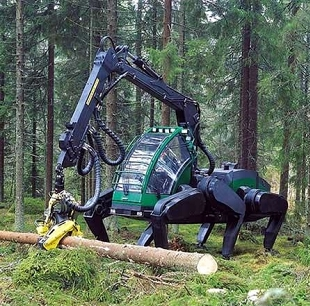
\includegraphics[width = 0.5\linewidth]{Introduction/intro18}
	\caption{Plustech Oy Ltd. Финляндия, 1999 г}
	\label{img:Plustech}
\end{figure}

На рисунках \ref{img:titan}---\ref{img:titan2} представлены японские разработки --- роботы семейства Titan.

\begin{figure}[ht]
	\begin{minipage}[ht]{0.49\linewidth}
		\centering{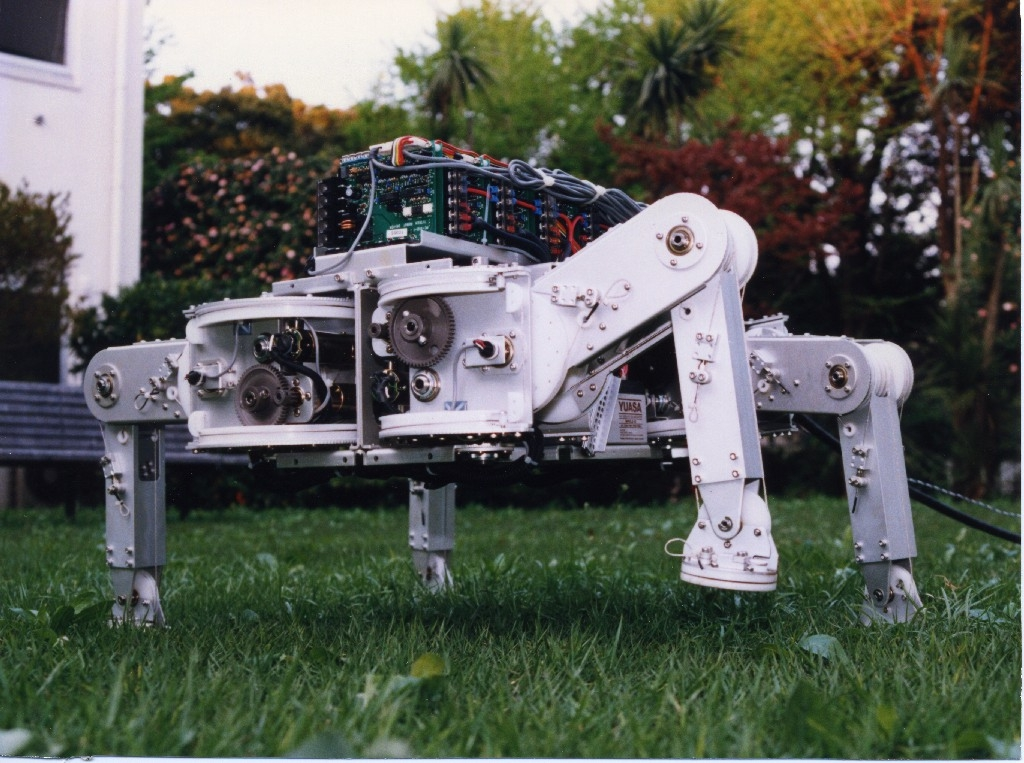
\includegraphics[width=0.8\linewidth]{Introduction/intro19} \\ а)}
	\end{minipage}
	\hfill
	\begin{minipage}[ht]{0.49\linewidth}
		\centering{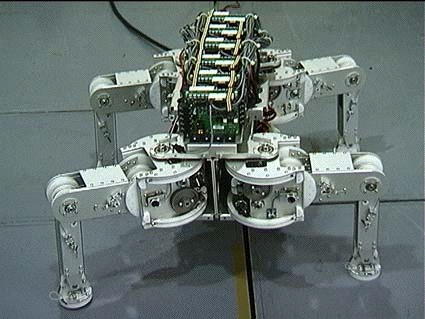
\includegraphics[width=0.8\linewidth]{Introduction/intro20} \\ б)}
	\end{minipage}
	\caption{Titan 8, Япония, Лаборатория профессора Хиросе}
	\label{img:titan}  
\end{figure}

\begin{figure}[ht]
	\centering
	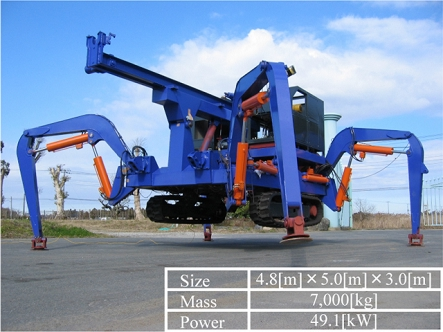
\includegraphics[width = 0.5\linewidth]{Introduction/intro21}
	\caption{Titan 11, Япония, Лаборатория профессора Хиросе}
	\label{img:titan2}
\end{figure}

На рис. \ref{img:lauron}---\ref{img:silo} представлены разработки Германии и Испании --- роботы семейств Lauron и Silo соответственно.

\begin{figure}[ht]
	\begin{minipage}[ht]{0.49\linewidth}
		\centering{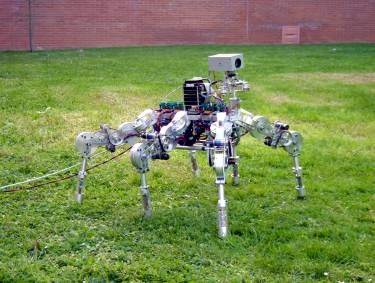
\includegraphics[width=0.8\linewidth]{Introduction/intro22} \\ а)}
	\end{minipage}
	\hfill
	\begin{minipage}[ht]{0.49\linewidth}
		\centering{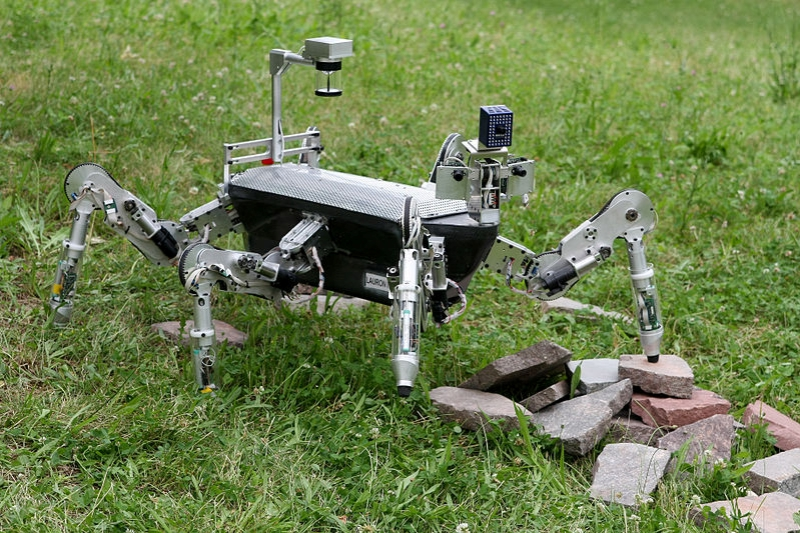
\includegraphics[width=0.8\linewidth]{Introduction/intro23} \\ б)}
	\end{minipage}
	\caption{Lauron 3, Lauron 4. Германия}
	\label{img:lauron}
\end{figure}

\begin{figure}[ht]
	\begin{minipage}[ht]{0.49\linewidth}
		\centering{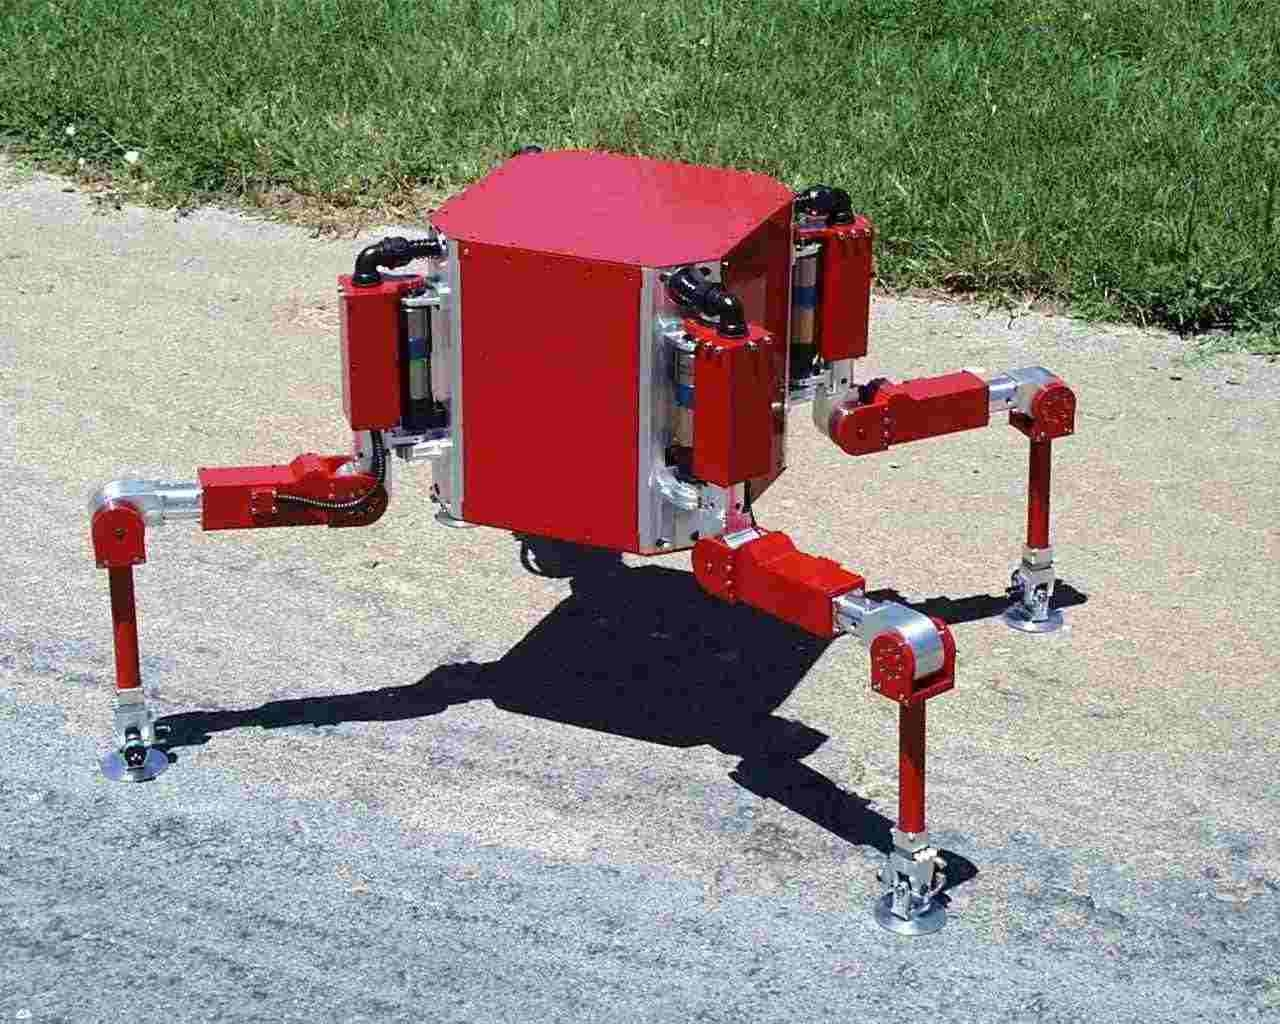
\includegraphics[width=0.8\linewidth]{Introduction/intro24} \\ а)}
	\end{minipage}
	\hfill
	\begin{minipage}[ht]{0.49\linewidth}
		\centering{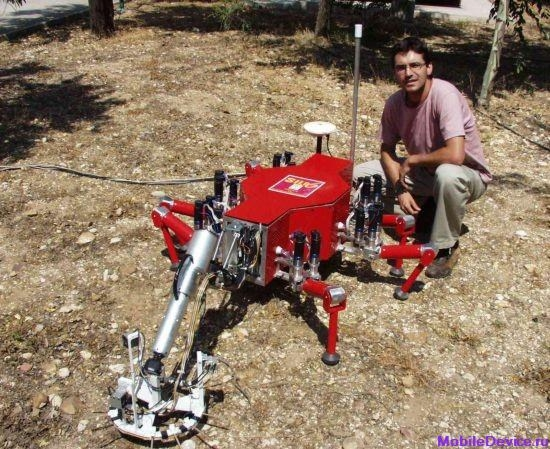
\includegraphics[width=0.8\linewidth]{Introduction/intro25} \\ б)}
	\end{minipage}
	\caption{Silo 4, Silo 6. Испания}
	\label{img:silo}
\end{figure}


На рис. \ref{img:bigdog} изображены самые современные аппараты --- хорошо известные Big Dog и Alpha Dog.

\begin{figure}[ht]
	\begin{minipage}[ht]{0.49\linewidth}
		\centering{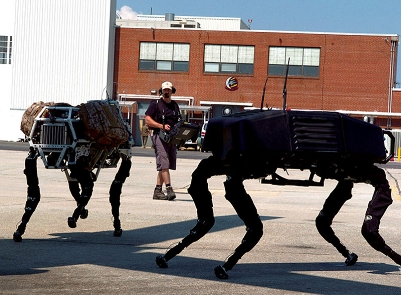
\includegraphics[width=0.8\linewidth]{Introduction/intro26} \\ а)}
	\end{minipage}
	\hfill
	\begin{minipage}[ht]{0.49\linewidth}
		\centering{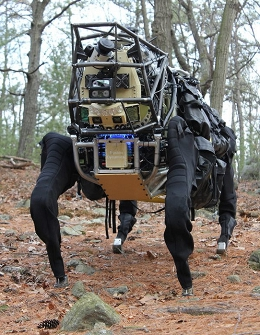
\includegraphics[width=0.8\linewidth]{Introduction/intro27} \\ б)}
	\end{minipage}
	\caption{Big Dog, Alpha Dog. США}
	\label{img:bigdog}
\end{figure}

На базе Волгоградского Государственного Технического Университета (ВолГТУ) создаются многоногие шагающие машины с ортогональной кинематикой ног и аппараты с циклическими механизмами ходьбы на основе механизмов схожих с лямбда-механизмами П.Л. Чебышева. На рис. \ref{img:octonog} изображена шагающая машина Восьминог. В кинематике аппарата параметры шагового цикла движения ноги-понтона определяются исключительно конструкцией ноги. 

\begin{figure}[ht]
	\begin{minipage}[ht]{0.49\linewidth}
		\centering{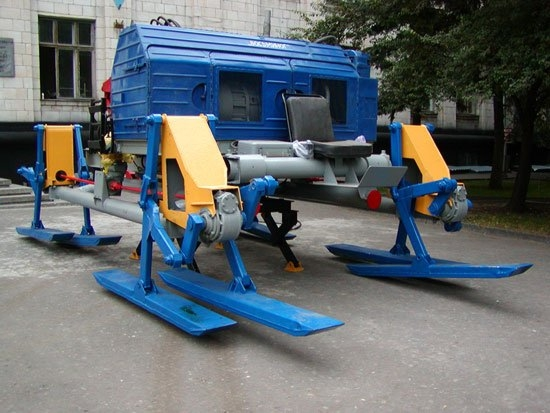
\includegraphics[width=0.8\linewidth]{Introduction/intro28} \\ а)}
	\end{minipage}
	\hfill
	\begin{minipage}[ht]{0.49\linewidth}
		\centering{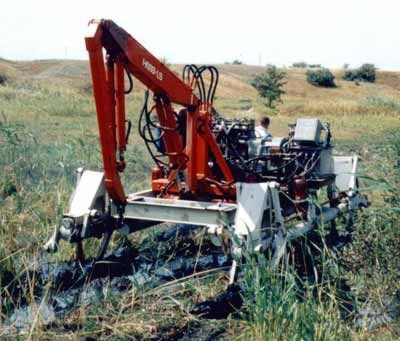
\includegraphics[width=0.8\linewidth]{Introduction/intro29} \\ б)}
	\end{minipage}
	\caption{Восьминог, ВолГТУ, Волгоград}
	\label{img:octonog}
\end{figure}

Малое количество подвижностей в в ногах аппарата ограничивает адаптационные возможности. С другой стороны, система управления аппаратом сильно упрощается. Машина Восьминог с ногами-понтонами способна передвигаться по очень слабым грунтам (рис. \ref{img:octonog}).

На рис. \ref{img:ortho} изображен макет аппарата с оригинальной кинематикой. Аппарат состоит из двух четырехногих модулей. Каждая нога аппарата выдвигается и убирается при помощи отдельного электродвигателя и штокового механизма. Четырехногие модули аппарата связаны между собой при помощи специального шарнира с одной вращательной степенью подвижности и одной поступательной степенью подвижности. Четырехногие модули по очереди находятся в опорной фазе. Пока один модуль находится в опоре, второй переносится в опорную область при помощи межмодульного шарнира. Систему управления для данного макета разрабатывалась в ИПМ им.М.В.Келдыша РАН.

\begin{figure}[ht]
	\centering
	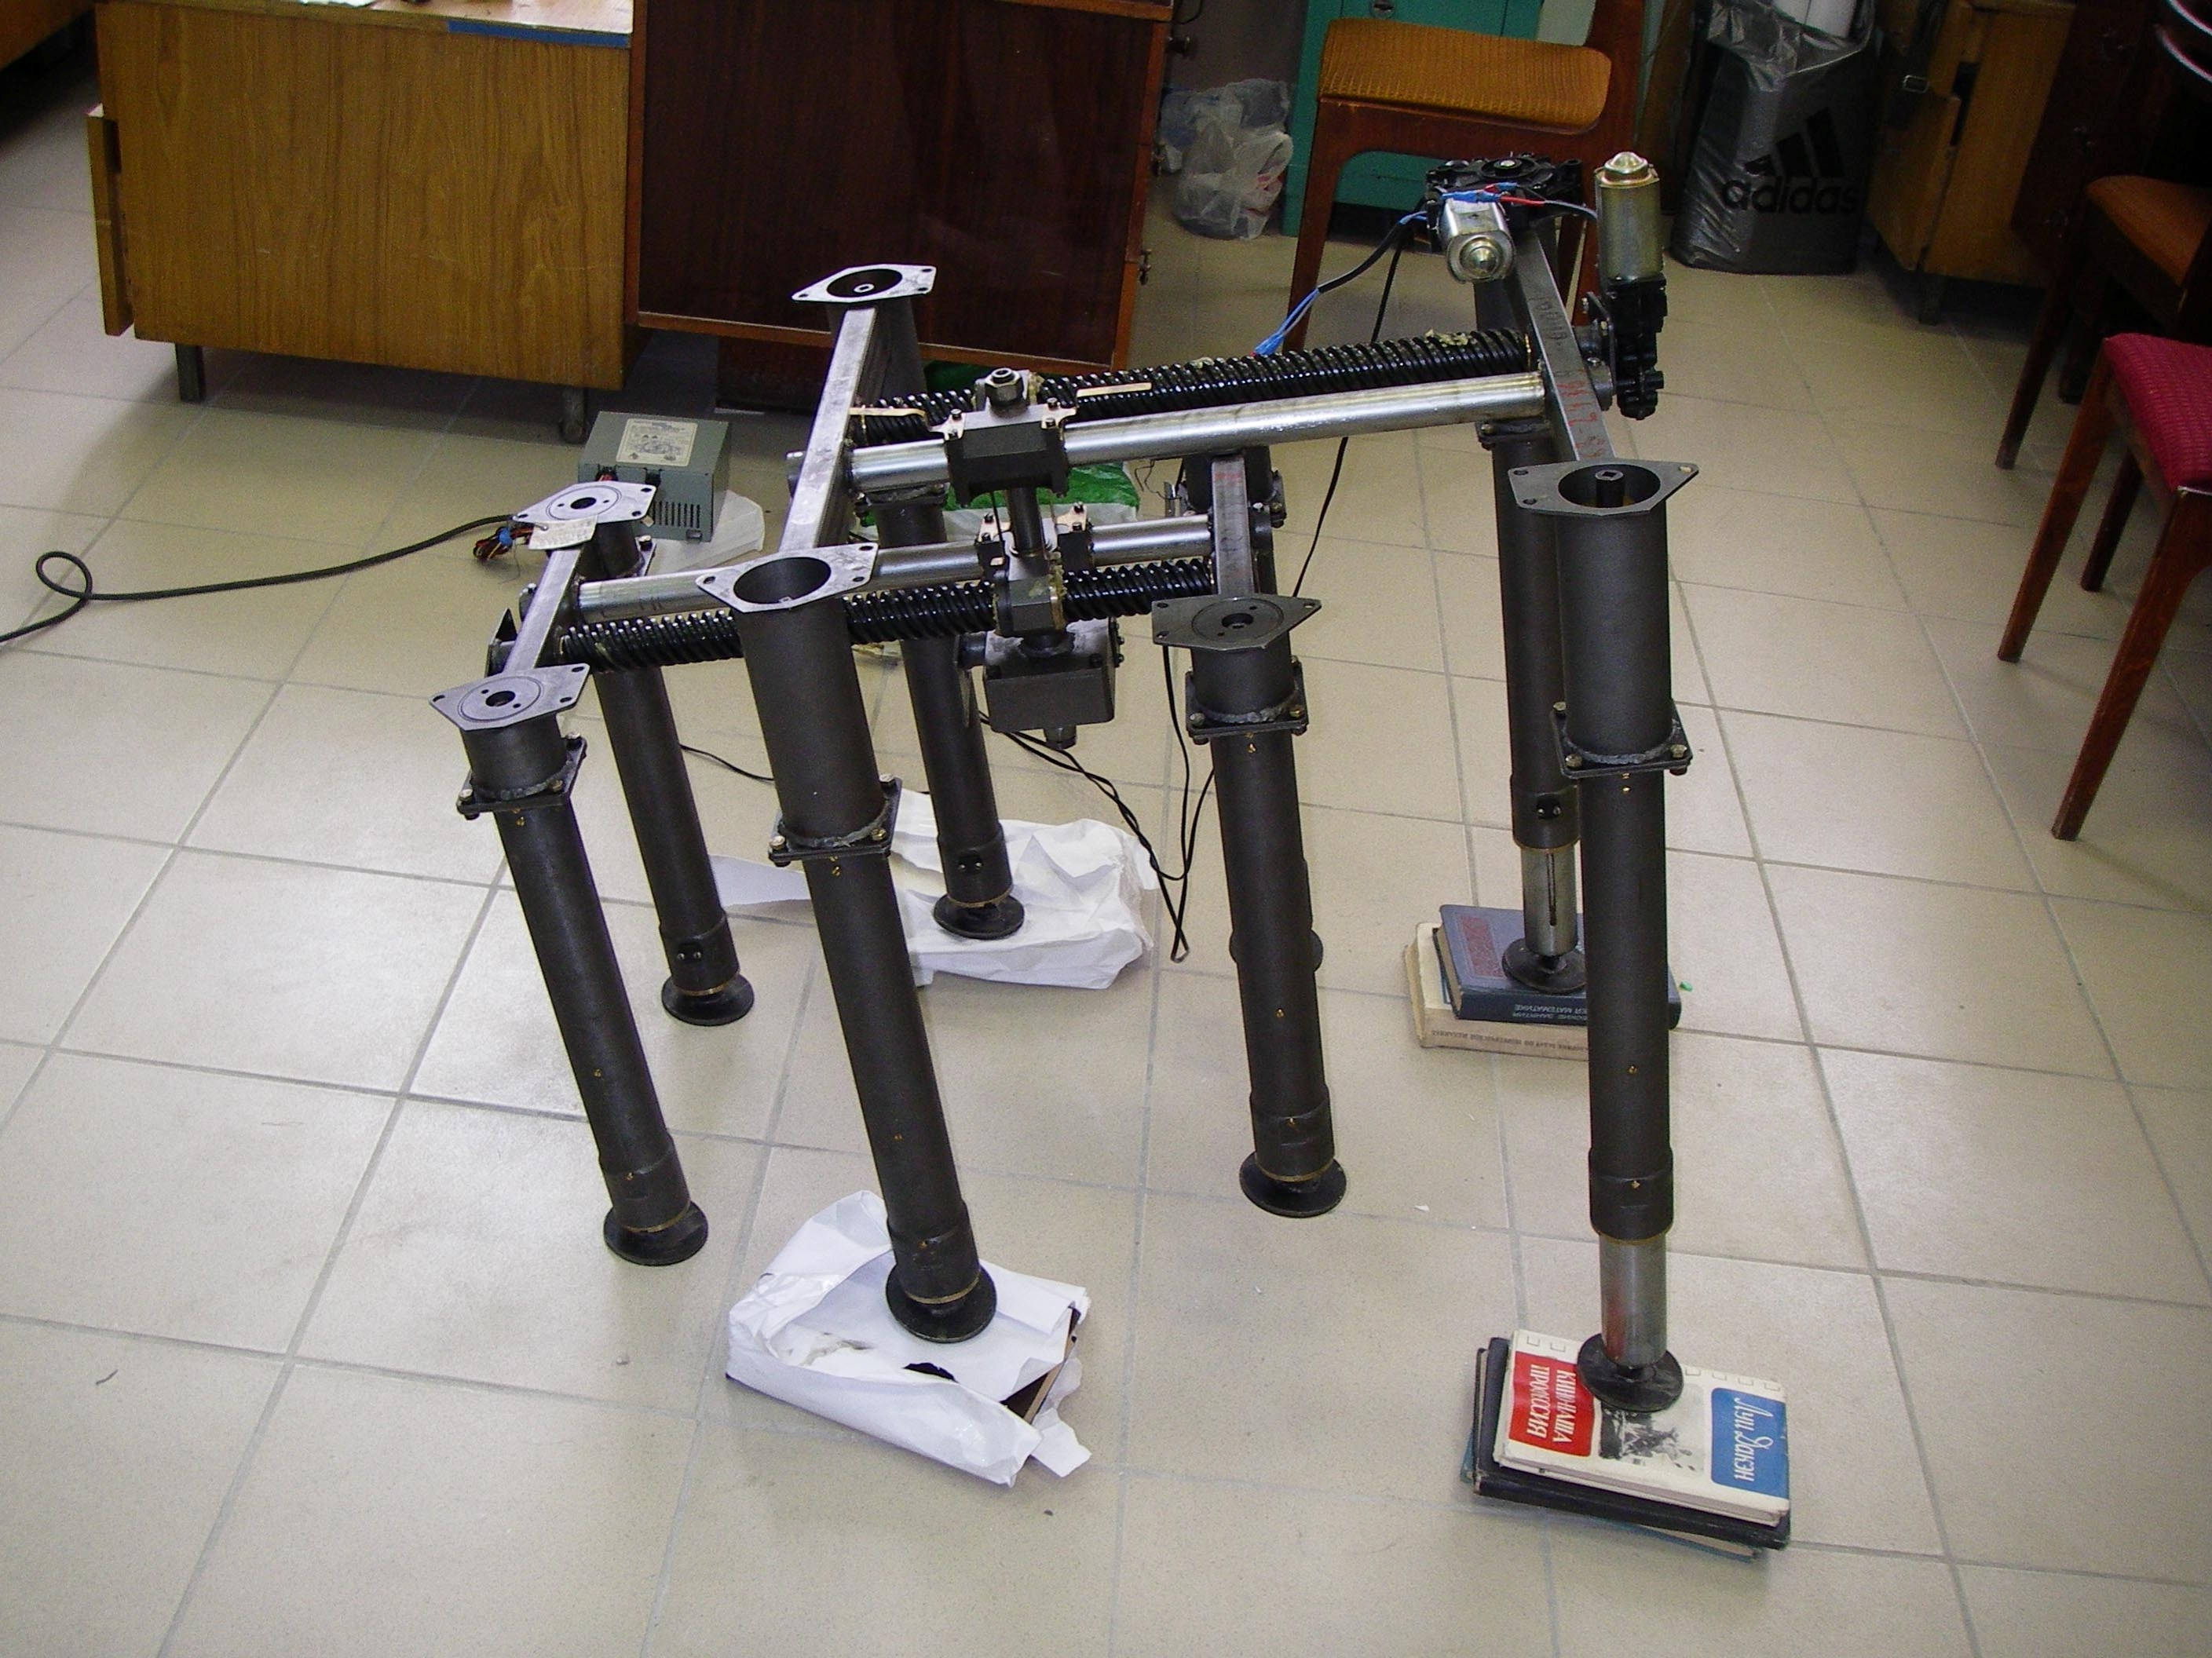
\includegraphics[width = 0.5\linewidth]{Introduction/intro30}
	\caption{}
	\label{img:ortho}
\end{figure}

На базе ВолГТУ выполняется проект по созданию большой восьминогой шагающей машины. На рис. \ref{img:ortho2} изображен действующий макет аппарата.

\begin{figure}[ht]
	\centering
	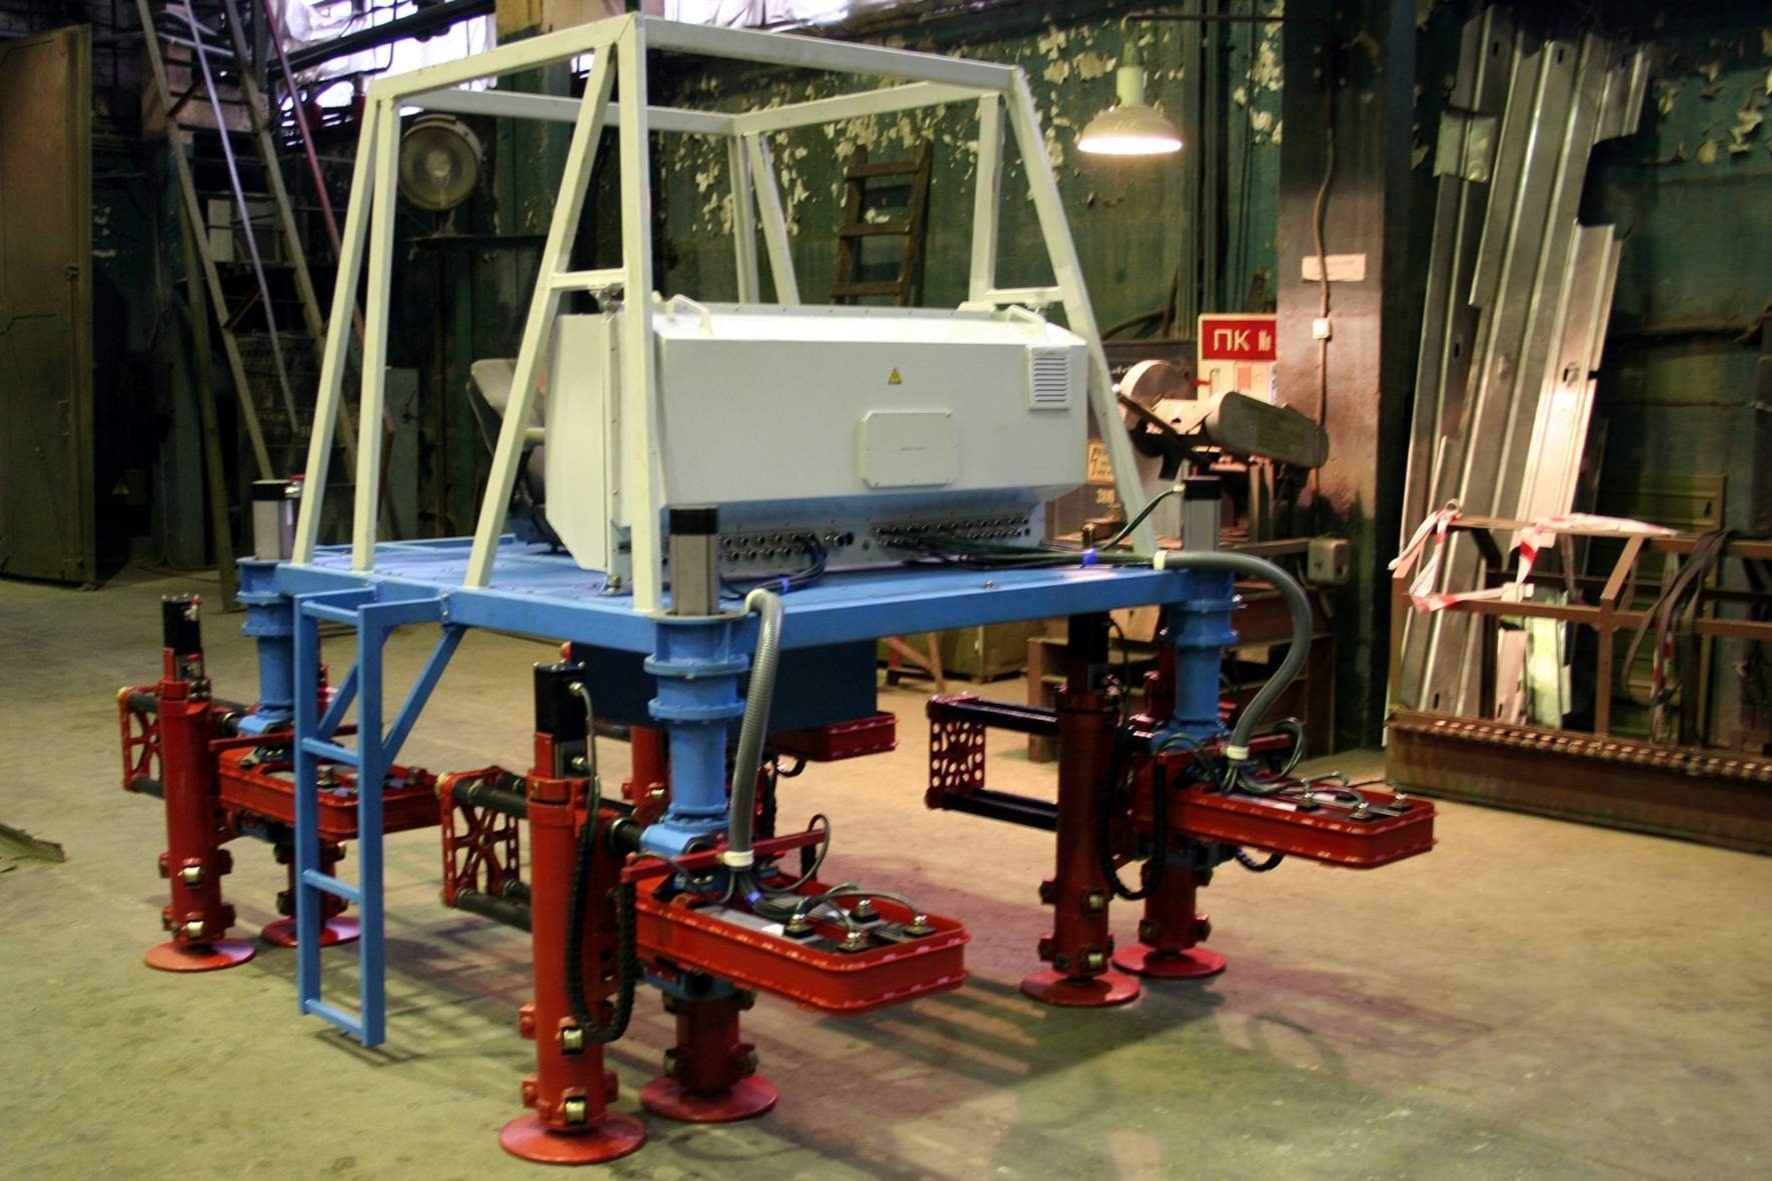
\includegraphics[width = 0.5\linewidth]{Introduction/intro31}
	\caption{Шагающая машина Ортоног, Волгоград}
	\label{img:ortho2}
\end{figure}

Машина состоит из корпуса и четырех пар ног с ортогональной кинематикой. Каждая пара ног связана между собой общей базой к которой крепятся горизонтальные штоки. Общая база пары ног соединена через поворотный механизм с корпусом аппарата.